\documentclass[a4paper,10pt]{article}
%\documentclass[a4paper,10pt]{scrartcl}

\usepackage[utf8]{inputenc}
%\usepackage{listings}
\usepackage{tikz}

\usetikzlibrary{arrows,automata}


\title{TP3 ACT}
\author{Matthieu Caron et Armand Bour}
\date{vendredi 9 octobre 2015}

\pdfinfo{%
  /Title    (TP2 ACT)
  /Author   (Matthieu Caron et Armand Bour)
  /Creator  (Matthieu Caron et Armand Bour)
  %/Producer ()
  %/Subject  ()
  %/Keywords ()
}

\begin{document}
\maketitle

\paragraph{Question 1}

Le code du graphique tikz est donné par Antoine Amara, mais la reflexion vient de nous 3.

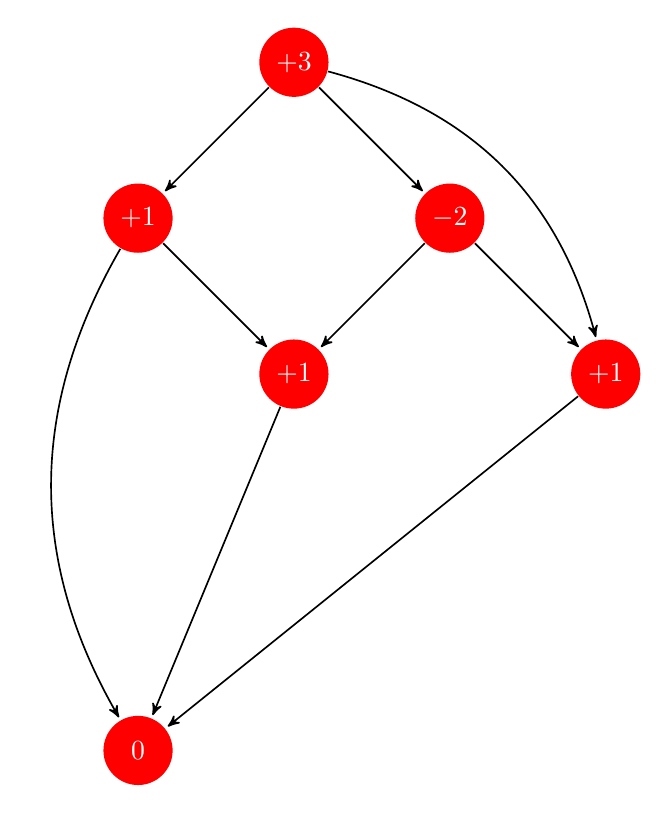
\begin{tikzpicture}[->,>=stealth',shorten >=1pt,auto,node distance=2.8cm,semithick]
    \tikzstyle{every state}=[fill=red,draw=none,text=white]
    \node[state] (A) {$+3$};
    \node[state] (B)[below left of=A] {$+1$};
    \node[state] (C)[below right of=A] {$-2$};
    \node[state] (D)[below left of=C] {$+1$};
    \node[state] (E)[below right of=C] {$+1$};
    \node[state] (F)[below of=D][below left of=E][below right of=B] {$0$};

    \path (A) edge              node {} (B)
    (B) edge                  node {} (D)
    (A) edge              node {} (C)
    (C) edge              node {} (D)
    (C) edge          node {} (E)
    (A) edge [bend left]         node {} (E)
    (B) edge [bend right]        node {} (F)
    (E) edge                     node {} (F)
    (D) edge                     node {} (F);
\end{tikzpicture}


\paragraph{Question 2}
Si ils sont tous positifs : $res = -1 * min(successeurs)-1$\newline
Sinon : $res = -1*max(desValeursNegatives) + 1$

\paragraph{Question 4}
Alors on utilise python, et on ne sait pas pourquoi la version dynamique prend beaucoup de temps,
avec des print on a compté, l'initialisation du tableau pour dynamic(100,100,50,50) dure une dizaine de secondes.

Donc dynamic(100,100,50,50) = -198.0
et dynamic(100,100,48,52) = 

Sinon on sait que c est beaucoup plus rapide que la version naive car naif(10,7,7,3) dure : real 4m2.556s
et dynamic(10,7,7,3) dure : real 0m0.120s.

\paragraph{Question 5}
pas faite

\paragraph{Question 6}
Alors on fait d'abord le remplissage du tableau qui dépend de $m$,$n$,$i$ et $j$ ce qui nous fait du $O(m*n*i*j)$
En suite dans l'algo on veut faire tous les découpages possible donc les decoupages dans la largeur $m$, et les decoupages dans la longueur $n$.
Donc si c est déjà calculé c est un acces au tableau on suppose en $O(1)$, on dis qu'on suppose car on ne connait pas l'objet ndarray en python est on a pas trouvé 
d'informations pour la complexité. Sinon c est le calcule de toutes les sous plaques de chocolat.

\[
\left \{
\begin{array}{c}
    \mathsf{si\: deja\: calc\: alors}\: c(m,n) = 1 \\
    \mathsf{sinon} \sum_{k=1}^m c(m-k,n) + \sum_{l=1}^n c(m,n-l) 
\end{array}
\right.
\]

la complexité est en $O(m^2*n^2)$

\paragraph{Question 7}
Toutes ces configurations ont la même valeur car c est la même plaque de chocolat soit tournée 1/4, 2/4, 3/4 de cercle ou vu de dos (symétrique)

\paragraph{Question 8}
L'idée c'est d'ajouter quand c est possible 8 valeurs au tableau plutot qu'une seule (la valeur habituelle et les 7 autres configurations identique).
On a testé pour (30,30,10,8), le dynamic simple dure : real 0m3.910s et le dynamic symetric dure : real 0m1.780s




\end{document}
